\subsection{Object Modeling}
Object modeling is essential to understand the static structure of the system . In this project, the system is designed to allow small shop owners to manage their products \& products efficiently. Object modeling is represented through class diagrams and object diagrams.

\noindent\textbf{Class Diagram:} The class diagram below represents the main classes, their attributes, methods, and relationships within the system.

\begin{figure}[H]
    \centering
    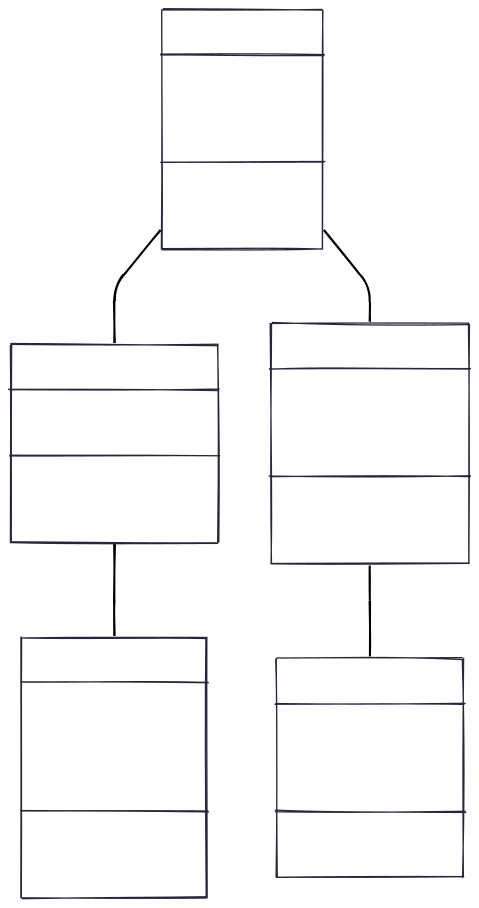
\includegraphics[width=0.7\textwidth]{diagrams/class-diagram.png}
    \caption{Class Diagram of the E-commerce System for SMEs}
\end{figure}

\noindent\textbf{Description of Main Classes:}

\begin{itemize}[nolistsep,leftmargin=*]
    \item \textbf{User:} Represents all system users including shop owners and customers. Attributes include userID, name, email, and methods like login(), logout(), updateProfile().
    \item \textbf{Product:} Represents items available for sale. Attributes include productID, name, price, stock, and methods such as addProduct(), updateProduct(), removeProduct().
    \item \textbf{Order:} Captures customer orders. Attributes include orderID, date, status, and methods like createOrder(), cancelOrder(), updateStatus().
    \item \textbf{Payment:} Handles transactions. Attributes include paymentID, amount, method, with methods processPayment(), refundPayment().
    \item \textbf{Cart:} Represents shopping cart. Attributes include cartID, items, and methods like addItem(), removeItem(), calculateTotal().
\end{itemize}

\noindent\textbf{Object Diagram:} To illustrate the runtime scenario, consider an example where a customer places an order. The object diagram demonstrates the relationships between specific instances of classes at that point in time.

\begin{figure}[H]
    \centering
    \includegraphics[width=1\textwidth]{diagrams/object-diagram.png}
    \caption{Object Diagram}
\end{figure}
\pagebreak

\noindent\textbf{Description of Objects:}

\begin{itemize}[nolistsep,leftmargin=*]
    \item \textbf{customer1:User} – Represents a specific customer instance.
    \item \textbf{cart1:Cart} – The cart object linked to customer1.
    \item \textbf{productA:Product, productB:Product} – Products added to cart1.
    \item \textbf{order1:Order} – Generated when the customer confirms the purchase.
    \item \textbf{payment1:Payment} – Associated with order1 for transaction processing.
\end{itemize}

\para{
This modeling helps visualize the structure and behavior of the system, ensuring clear understanding of entity relationships and interactions before implementation. It also provides a foundation for refining class methods, attributes, and their interconnections during system design.
}
